\chapter{Algoritmos Divide y Vencerás: \textit{The Skyline problem}}

\section{Enunciado al problema de la línea del horizonte}

\begin{displayquote}
Tengamos un conjunto de $n$ rectángulos en un orden arbitrario formado por rectángulos de altura y anchura variables pero cuyas bases son colineares, de forma que parecn edificios en un \textit{skyline}.
Para cada rectángulo tenemos la posición $x$ del extremo izquierdo y el derecho y su altura.
Se pide dibujar una línea alrededor del conjunto de rectángulos de forma que se pueda ver el \textit{skyline} de la misma forma que se vería en silueta por la noche (Gordon, 2014).
\end{displayquote}

\begin{figure}[h]
\begin{center}
	
\includegraphics[scale=0.4]{TrabajoAutonomo/Rectangulos}
	\caption{Estado inicial del problema: Rectángulos de características arbitrarias (Gordon, 2014)}
\end{center}
\end{figure}

\begin{figure}[h]
\begin{center}
	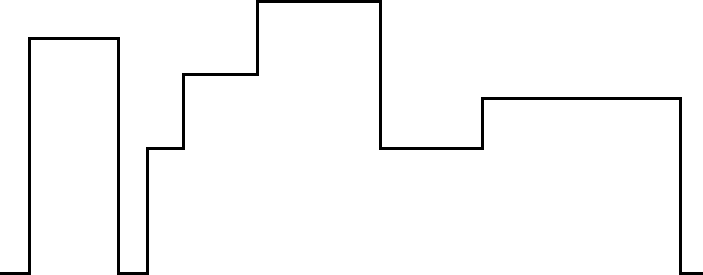
\includegraphics[scale=0.4]{TrabajoAutonomo/Skyline}
	\caption{Estado final del problema: Línea del horizonte (Gordon, 2014)}
\end{center}
\end{figure}

\pagebreak

\section{Algoritmo básico de resolución}

Para resolver este problema vamos a trabajar con un vector \code{skyline} de $n$ elementos, entre los cuales podrán posicionarse los rectángulos de sin excederse de los límites mayor y menor de dicho vector.
Cada rectángulo está formado por tres variables:

\begin{itemize}
	\item\code{Altura}\textbf{:} Número de bloques de elevación sobre la base.
	\item\code{Anchura}\textbf{:} Número de bloques que se extiende el rectángulo hacia valores positivos del eje $x$.
	\item\code{Posición}\textbf{:} Índice del bloque de valores positivos del eje $x$ en el que comienza el rectángulo.
\end{itemize}

Dada una lista de rectángulos definidos con estas variables, la recorremos secuencialmente analizando la altura máxima de cada posición en base a si la altura del rectángulo en una posición del vector \code{skyline} es mayor a la altura máxima registrada en el mismo.
Antes de empezar, todas las posiciones del vector están inicializadas a $0$.

Expresado en pseudocódigo tenemos el siguiente algoritmo:

\begin{lstlisting}[language = Python]
for rectangulo in lista_rectangulos:
	for i in rectangulo->posicion..rectangulo->(posicion+anchura):
		if rectangulo->altura > skyline[i]:
			skyline[i] = rectangulo->altura
\end{lstlisting}

\subsection{Eficiencia del algoritmo básico}

Este algoritmo contiene un bucle anidado dentro de otro.
El bucle interno contiene una sentencia condicional cuya comprobación y cuerpo son operaciones elementales, por lo que su eficiencia es $O(1)$.
Tanto la inicialización como la comprobación y actialización de los bucles interno y externo son todas operaciones elementales, por lo que la eficiencia de todas ellas es $O(1)$.
El bucle interno se ejecuta tantas veces como posiciones tenga el rectángulo al que se refiere, siendo su eficiencia $O(n)$.
El bucle externo se ejecuta tantas veces como rectángulos contenga el problema, siendo su eficiencia $O(n)$.
Teniendo en cuenta estos datos y por la regla del producto, la eficiencia total de este algoritmo es $O(n^2)$.

\section{Algoritmo Divide y Vencerás}

\section{Implementación de ambos algoritmos}

\section{Posibles mejoras del algoritmo}
